\documentclass[10pt,aspectratio=169]{beamer}

\usetheme{Madrid}
\usecolortheme{default}
\usepackage{amsmath,amssymb}
\usepackage{tikz}
\usetikzlibrary{arrows.meta,positioning}

\setbeamertemplate{navigation symbols}{}
\setbeamertemplate{footline}{%
  \leavevmode%
  \hbox{%
    \begin{beamercolorbox}[wd=\paperwidth,ht=2.5ex,dp=1.2ex,leftskip=1em,rightskip=1em]{author in head/foot}%
    HKUST Optimizing Decisions for Personal and Business Development
    \hfill Birth-and-Death Practice Solution
    \end{beamercolorbox}}%
}

\title{Birth-and-Death Practice: Complete Solution}
\author{IEDA 1250}
\date{}

\begin{document}

\begin{frame}{Practice Solution: CTMC Diagram and Balance}
Given
\[
\lambda_0=3,\qquad \lambda_1=2,\qquad \lambda_2=1,\qquad
\lambda_n=0\ (n\geq 3),
\]
\[
\mu_n=2,\qquad n=1,2,\ldots
\]
Only states \(0,1,2,3\) can have positive steady-state probability.

\vspace{0.25cm}
\begin{center}
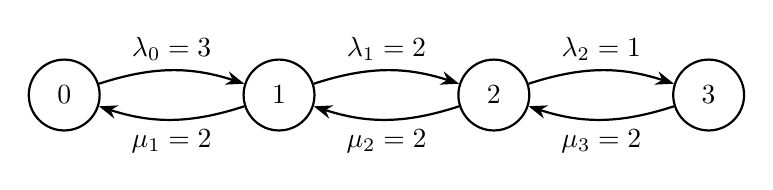
\begin{tikzpicture}[
  state/.style={circle,draw,minimum size=0.9cm,thick},
  >=Stealth,
  node distance=1.8cm
]
\node[state] (s0) {0};
\node[state,right=of s0] (s1) {1};
\node[state,right=of s1] (s2) {2};
\node[state,right=of s2] (s3) {3};
\draw[->,thick,bend left=18] (s0) to node[above] {\(\lambda_0=3\)} (s1);
\draw[->,thick,bend left=18] (s1) to node[below] {\(\mu_1=2\)} (s0);
\draw[->,thick,bend left=18] (s1) to node[above] {\(\lambda_1=2\)} (s2);
\draw[->,thick,bend left=18] (s2) to node[below] {\(\mu_2=2\)} (s1);
\draw[->,thick,bend left=18] (s2) to node[above] {\(\lambda_2=1\)} (s3);
\draw[->,thick,bend left=18] (s3) to node[below] {\(\mu_3=2\)} (s2);
\end{tikzpicture}
\end{center}

\vspace{0.15cm}
Local balance equations:
\[
3\pi_0=2\pi_1,\qquad 2\pi_1=2\pi_2,\qquad \pi_2=2\pi_3.
\]
\end{frame}

\begin{frame}{Practice Solution: Steady-State Probabilities}
From local balance,
\[
\pi_1=\frac{3}{2}\pi_0,
\qquad
\pi_2=\pi_1=\frac{3}{2}\pi_0,
\qquad
\pi_3=\frac{1}{2}\pi_2=\frac{3}{4}\pi_0.
\]

Use normalization:
\[
\pi_0+\pi_1+\pi_2+\pi_3=1.
\]
Substitute the expressions in terms of \(\pi_0\):
\[
\pi_0+\frac{3}{2}\pi_0+\frac{3}{2}\pi_0+\frac{3}{4}\pi_0=1.
\]
\[
\frac{19}{4}\pi_0=1
\quad \Rightarrow \quad
\pi_0=\frac{4}{19}.
\]
Therefore,
\[
\boxed{
\pi_0=\frac{4}{19},\quad
\pi_1=\frac{6}{19},\quad
\pi_2=\frac{6}{19},\quad
\pi_3=\frac{3}{19}
}
\]
and
\[
\boxed{\pi_n=0,\qquad n=4,5,\ldots}
\]
\end{frame}

\begin{frame}{Practice Solution: Effective Arrival Rate and Queue Size}
The effective arrival rate is
\[
\lambda_e=\sum_{n=0}^{\infty}\lambda_n\pi_n
=3\pi_0+2\pi_1+\pi_2
=\frac{12}{19}+\frac{12}{19}+\frac{6}{19}
=\frac{30}{19}.
\]

Expected number in the system:
\[
E[N]=\sum_{n=0}^{3}n\pi_n
=\frac{6}{19}+\frac{12}{19}+\frac{9}{19}
=\frac{27}{19}.
\]

For a single-server system, queue length in state \(n\) is \(\max\{n-1,0\}\). Thus,
\[
E[N_Q]=(0)\pi_1+(1)\pi_2+(2)\pi_3
=\frac{6}{19}+\frac{6}{19}
=\frac{12}{19}.
\]
\end{frame}

\begin{frame}{Practice Solution: Time Metrics}
By Little's Law with \(\lambda_e\),
\[
\boxed{E[T]=\frac{E[N]}{\lambda_e}
=\frac{27/19}{30/19}
=0.9}
\]
\[
\boxed{E[T_Q]=\frac{E[N_Q]}{\lambda_e}
=\frac{12/19}{30/19}
=0.4}
\]

\vspace{0.2cm}
Final answers:
\[
\boxed{
\pi_0=\frac{4}{19},\quad
\pi_1=\frac{6}{19},\quad
\pi_2=\frac{6}{19},\quad
\pi_3=\frac{3}{19},\quad
\pi_n=0\ (n\geq 4)
}
\]
\[
\boxed{
\lambda_e=\frac{30}{19},\quad
E[N]=\frac{27}{19},\quad
E[N_Q]=\frac{12}{19},\quad
E[T]=0.9,\quad
E[T_Q]=0.4
}
\]
\end{frame}

\end{document}
